\section{System Architecture}

The MediCare Secure RAG system is structured as a modular Python application orchestrated by \texttt{rag/pipeline.py}. The architecture separates three concerns: (1) the vulnerable baseline retrieval path used to demonstrate attacks, (2) the five-layer secured path, and (3) the Streamlit presentation layer. Figure \ref{fig:arch} shows the full data-flow diagram.

\begin{figure}[H]
\centering
\begin{tikzpicture}[
  node distance=0.55cm,
  box/.style={rectangle, draw=black!70, rounded corners=3pt, text centered,
              minimum width=9cm, minimum height=0.75cm, font=\small},
  ui/.style={box, fill=gray!20},
  orch/.style={box, fill=blue!12},
  defense/.style={box, fill=orange!20},
  gen/.style={box, fill=green!15},
  risk/.style={box, fill=gray!20},
  arrow/.style={->, thick, >=stealth}
]
  \node[ui]      (ui)   {Streamlit UI (\texttt{app.py})};
  \node[orch,    below=of ui]  (pipe) {Pipeline Orchestrator (\texttt{rag/pipeline.py})};
  \node[orch,    below=of pipe](ret)  {Retriever (\texttt{rag/retriever.py}) $\rightarrow$ ChromaDB};
  \node[defense, below=of ret] (l2)   {\textbf{Layer 2:} RBAC Access Control (runs 1st)};
  \node[defense, below=of l2]  (l1)   {\textbf{Layer 1:} Ingestion Sanitisation (runs 2nd)};
  \node[defense, below=of l1]  (l5)   {\textbf{Layer 5:} Embedding Anomaly Detection (runs 3rd)};
  \node[gen,     below=of l5]  (gen)  {Generator (\texttt{rag/generator.py}) + \textbf{Layer 3:} Prompt Hardening};
  \node[defense, below=of gen] (l4)   {\textbf{Layer 4:} Post-Generation Output Monitoring};
  \node[risk,    below=of l4]  (risk) {Risk Scorer + CRIR (\texttt{security/risk\_score.py})};

  \draw[arrow] (ui)   -- (pipe);
  \draw[arrow] (pipe) -- (ret);
  \draw[arrow] (ret)  -- (l2);
  \draw[arrow] (l2)   -- (l1);
  \draw[arrow] (l1)   -- (l5);
  \draw[arrow] (l5)   -- (gen);
  \draw[arrow] (gen)  -- (l4);
  \draw[arrow] (l4)   -- (risk);
\end{tikzpicture}
\caption{Data-flow architecture of MediCare Secure RAG. Orange boxes denote the five active defence layers. The RBAC layer (L2) runs first as a cheap metadata check, followed by sanitisation (L1), then anomaly detection (L5).}
\label{fig:arch}
\end{figure}

\section{Document Ingestion Pipeline}

\justifying

At startup, \texttt{rag/vector\_store.py} calls \texttt{init\_db()}, which deletes any existing ChromaDB collection and recreates it. Each document from \texttt{data/healthcare/clean\_docs.jsonl} undergoes the following processing steps:

\begin{enumerate}
    \item \textbf{Text extraction:} The \texttt{text} field is read from the JSONL record.

    \item \textbf{Embedding generation:} \texttt{rag/embedder.py} calls the Sentence-Transformers model to produce a 384-dimensional embedding vector.

    \item \textbf{Hash computation:} A SHA-256 content hash is computed for integrity verification.

    \item \textbf{Metadata tagging:} Fields \texttt{classification} (public/internal/restricted),
    \texttt{source}, \texttt{topic}, and \texttt{kind} are stored alongside the embedding in ChromaDB.
\end{enumerate}

\noindent
Poisoned documents are loaded identically via \texttt{inject\_poison()}, with their \texttt{attack\_type} field marking them as adversarial (used only for evaluation metrics, not by the defence layers themselves).

\section{Query and Retrieval Pipeline}

Figure \ref{fig:ragflow} illustrates the query-to-answer flow.

\begin{figure}[H]
\centering
\begin{tikzpicture}[
  main/.style={rectangle, draw=black!70, fill=blue!8, rounded corners=3pt,
               text centered, minimum width=6.5cm, minimum height=0.75cm, font=\small},
  defence/.style={rectangle, draw=black!70, fill=orange!18, rounded corners=3pt,
                  text centered, minimum width=4.8cm, minimum height=0.75cm, font=\small},
  decision/.style={diamond, draw=black!70, fill=yellow!25, text centered,
                   minimum width=3.0cm, inner sep=3pt, font=\small, aspect=2.5},
  arrow/.style={->, thick, >=stealth}
]
%% ---- Main vertical flow (centred at x=0) ----
\node[main]     at (0,    0)   (query)  {User Query + Role};
\node[main]     at (0, -1.2)   (embed)  {Embed Query (\texttt{all-MiniLM-L6-v2})};
\node[main]     at (0, -2.4)   (chroma) {ChromaDB Cosine Search $\to$ Top-5 Docs};
\node[decision] at (0, -3.8)   (def)    {Defence\\ON?};

%% ---- YES branch: three separate defence layers (left column, x=-5.2) ----
\node[defence]  at (-5.2, -5.1)  (l2)  {\textbf{Layer 2:} RBAC Access Control};
\node[defence]  at (-5.2, -6.1)  (l1)  {\textbf{Layer 1:} Ingestion Sanitisation};
\node[defence]  at (-5.2, -7.1)  (l5)  {\textbf{Layer 5:} Anomaly Detection};

%% ---- Main flow continues below decision ----
\node[main]     at (0, -8.6)   (gen)  {Generator (Groq API) + \textbf{Layer 3}};
\node[main]     at (0, -9.8)   (l4)   {\textbf{Layer 4:} Output Monitor};
\node[main]     at (0,-11.0)   (risk) {CRIR + Composite Risk Score};
\node[main]     at (0,-12.2)   (ui)   {Return Result to UI};

%% ---- Arrows: main flow ----
\draw[arrow] (query)  -- (embed);
\draw[arrow] (embed)  -- (chroma);
\draw[arrow] (chroma) -- (def);

%% ---- YES: left from diamond → down through L2 → L1 → L5 ----
\draw[arrow] (def.west)
    -- node[above, font=\scriptsize]{Yes}
    (-5.2, -3.8)          %% horizontal segment at diamond level
    -- (l2.north);        %% down to Layer 2
\draw[arrow] (l2) -- (l1);
\draw[arrow] (l1) -- (l5);

%% L5 south → down to gen y-level → right into gen.west
\draw[arrow] (l5.south)
    -- (-5.2, -8.6)       %% straight down to gen's y
    -- (gen.west);        %% right into Generator

%% ---- NO: straight down from diamond to Generator ----
\draw[arrow] (def.south)
    -- node[right, font=\scriptsize]{No}
    (gen.north);

%% ---- Continue main flow ----
\draw[arrow] (gen)  -- (l4);
\draw[arrow] (l4)   -- (risk);
\draw[arrow] (risk) -- (ui);
\end{tikzpicture}
\caption{RAG query-to-answer pipeline. When Defence is ON (left branch), retrieved
         documents pass sequentially through Layer~2 (RBAC), Layer~1 (Sanitisation),
         and Layer~5 (Anomaly Detection) before reaching the Generator.
         When Defence is OFF (right branch), documents go directly to the Generator.}
\label{fig:ragflow}
\end{figure}

The retriever (\texttt{rag/retriever.py}) performs pure cosine similarity search. Given a query $q$:
\begin{equation}
\text{score}(q, d_i) = \frac{\vec{q} \cdot \vec{d_i}}{|\vec{q}||\vec{d_i}|}
\end{equation}
The top-$k=5$ documents by cosine score are returned with \textbf{no access control or filtering} by design --- this is the intentionally vulnerable baseline.

\section{Anti-Poisoning Architecture: The Five-Layer Defence Pipeline}

Figure \ref{fig:pipeline} illustrates the sequential execution of all five defence layers. Critically, the execution order is \textbf{Layer 2 $\to$ Layer 1 $\to$ Layer 5} at the retrieval stage (in \texttt{defense\_filter()}), followed by Layer 3 at generation time, and Layer 4 post-generation. Layer 2 runs first because a simple metadata check is cheaper than regex scanning and immediately eliminates all unauthorised documents before Layer 1 spends cycles analysing them.

\begin{figure}[H]
\centering
\begin{tikzpicture}[
  node distance=0.45cm,
  layer/.style={rectangle, draw=black!60, rounded corners=4pt, text centered,
                minimum width=10cm, text width=9.8cm, minimum height=1.0cm,
                font=\small\bfseries},
  sub/.style={rectangle, draw=black!30, fill=gray!5, rounded corners=2pt,
              minimum width=10cm, text width=9.8cm, minimum height=0.65cm,
              text centered, font=\footnotesize},
  divider/.style={rectangle, draw=black!20, fill=gray!10, rounded corners=2pt,
                  minimum width=10cm, text width=9.8cm, minimum height=0.5cm,
                  text centered, font=\footnotesize\itshape},
  arrow/.style={->, thick, >=stealth}
]
  %% --- RETRIEVAL STAGE (L2, L1, L5) ---
  \node[layer, fill=orange!30] (l2)  {Layer 2: RBAC Access Control \textnormal{(retrieval, runs 1st)}};
  \node[sub,   below=of l2]    (l2s) {Blocks docs where classification $\notin$ role's allowed levels (patient $\to$ public only)};
  \node[layer, fill=orange!20, below=0.3cm of l2s] (l1)  {Layer 1: Ingestion Sanitisation \textnormal{(retrieval, runs 2nd)}};
  \node[sub,   below=of l1]    (l1s) {Strips 8 marker patterns; blocks 5 semantic injection phrases};
  \node[layer, fill=orange!20, below=0.3cm of l1s] (l5)  {Layer 5: Embedding Anomaly Detection \textnormal{(retrieval, runs 3rd)}};
  \node[sub,   below=of l5]    (l5s) {Pairwise cosine similarity within topic groups; blocks coordinated injections (cosine $>$ 0.70, untrusted source)};

  %% --- GENERATION STAGE (L3 inside Generator, then L4) ---
  \node[divider, below=0.4cm of l5s] (div) {--- Generation Stage ---};
  \node[layer, fill=green!20,  below=0.3cm of div]  (l3)  {Layer 3: Prompt Hardening \textnormal{(in Generator)}};
  \node[sub,   below=of l3]    (l3s) {Positional prompt fencing; each retrieved doc isolated with unique markers; 4 anti-injection safety rules prepended};
  \node[layer, fill=red!20,    below=0.3cm of l3s] (l4)  {Layer 4: Post-Generation Output Monitoring};
  \node[sub,   below=of l4]    (l4s) {8 danger regex patterns; HIGH severity $\to$ response blocked; MEDIUM $\to$ flagged};

  \draw[arrow] (l2)  -- (l2s);
  \draw[arrow] (l2s) -- (l1);
  \draw[arrow] (l1)  -- (l1s);
  \draw[arrow] (l1s) -- (l5);
  \draw[arrow] (l5)  -- (l5s);
  \draw[arrow] (l5s) -- (div);
  \draw[arrow] (div) -- (l3);
  \draw[arrow] (l3)  -- (l3s);
  \draw[arrow] (l3s) -- (l4);
  \draw[arrow] (l4)  -- (l4s);
\end{tikzpicture}
\caption{The five-layer defence pipeline in correct execution order: Layers 2, 1, and 5 operate at the retrieval stage (filtering documents before generation); Layer 3 operates inside the Generator (hardening the prompt); Layer 4 operates post-generation (monitoring the LLM output).}
\label{fig:pipeline}
\end{figure}




\subsection{Layer 1 --- Ingestion Sanitisation}
Implemented in \texttt{defense.py::layer1\_sanitize()}. Scans document text for embedded injection markers using two categories of compiled regex patterns:
\begin{itemize}
    \item \textbf{Marker-based patterns:} HTML comments, \texttt{[SYSTEM]...[/SYSTEM]} blocks, \texttt{---SYSTEM---} delimiters, and ``ignore previous instructions'' phrases. Detected markers are stripped and the document is retained with a \texttt{\_sanitized} flag.
    \item \textbf{Semantic injection patterns:} Authoritative-sounding instruction phrases. Documents matching these patterns are blocked entirely.
\end{itemize}

\subsection{Layer 2 --- Role-Based Access Control at Retrieval}
Implemented in \texttt{defense.py::layer2\_access\_control()}. Enforces a three-tier classification model. This layer runs \textbf{first} in \texttt{defense\_filter()} as a low-cost metadata check:
\begin{itemize}
    \item \textbf{patient} $\rightarrow$ access to \texttt{public} documents only.
    \item \textbf{nurse} $\rightarrow$ access to \texttt{public} and \texttt{internal} documents.
    \item \textbf{doctor} $\rightarrow$ access to \texttt{public}, \texttt{internal}, and \texttt{restricted} documents.
\end{itemize}

\subsection{Layer 3 --- Hardened Prompt Template}
Implemented in \texttt{rag/generator.py}. The secure prompt wraps each retrieved document in plain-text positional fences (\texttt{[REFERENCE DOCUMENT \{i\} - START]} ... \texttt{[REFERENCE DOCUMENT \{i\} - END]}) and prepends four explicit critical rules instructing the model to treat the document content as data, never as instructions.

\subsection{Layer 4 --- Post-Generation Output Monitoring}
Implemented in \texttt{defense.py::layer4\_monitor\_output()}. Scans the LLM response for eight danger patterns using compiled regular expressions including: suspicious URLs, system prompt leak indicators, API key patterns, unsafe paracetamol dosages ($\geq$8,000\,mg/day), incorrect heart rate ranges, and context exfiltration templates.

\subsection{Layer 5 --- Embedding-Level Anomaly Detection}
Implemented in \texttt{defense.py::layer5\_anomaly\_detect()}. Detects coordinated injection (the PoisonedRAG pattern) by:
\begin{enumerate}
    \item Grouping retrieved documents by \texttt{topic} metadata field.
    \item Computing pairwise cosine similarities within each topic group.
    \item Flagging pairs with similarity $>$ 0.70 whose \texttt{source} is not in the trusted allowlist.
\end{enumerate}

\section{Database Design}

Each document in the ChromaDB collection is stored with the following field schema:

\begin{longtable}{|p{3.2cm}|p{2.5cm}|p{7.3cm}|}
\caption{ChromaDB Document Schema in MediCare Secure RAG.}
\label{tab:dbschema} \\
\hline
\rowcolor{gray!15}
\textbf{Field} & \textbf{Type} & \textbf{Description} \\
\hline
\endfirsthead
\multicolumn{3}{l}{\small\textit{Table \thetable{} continued from previous page}} \\[2pt]
\hline
\rowcolor{gray!15}
\textbf{Field} & \textbf{Type} & \textbf{Description} \\
\hline
\endhead
\hline
\endlastfoot
\texttt{id}            & string     & Unique document identifier (e.g., \texttt{med-001}) \\
\hline
\texttt{text}          & string     & Full document content (ChromaDB documents field) \\
\hline
\texttt{topic}         & string     & Medical topic used by Layer~5 grouping \\
\hline
\texttt{classification}& string     & Access level: \texttt{public}, \texttt{internal}, or \texttt{restricted} \\
\hline
\texttt{source}        & string     & Source identifier for Layer~5 trusted allowlist \\
\hline
\texttt{attack\_type} & string     & Empty for clean docs; attack class for poisoned docs \\
\hline
\texttt{safe}          & boolean    & \texttt{True} for clean documents; \texttt{False} for poisoned \\
\hline
\texttt{content\_hash}& string     & SHA-256 hash of document text for integrity verification \\
\hline
\texttt{\_embedding}  & list[float]& 384-dimensional sentence embedding vector \\
\hline
\end{longtable}

\section{Authentication and Access Control Sequence}

For a patient-role query the access control flow is:
\begin{enumerate}
    \item UI receives query; role set to \texttt{patient}.
    \item Retriever returns top-5 documents with no filtering.
    \item Layer 2 iterates: documents with \texttt{classification} $\neq$ \texttt{public} are moved to \texttt{blocked\_docs}.
    \item Only \texttt{public} documents proceed to Layer 1.
    \item Layer 1 removes or strips injection markers.
    \item Layer 5 removes coordinated-injection outliers.
    \item Remaining documents are passed to the generator with Layer 3 prompt hardening.
\end{enumerate}

\section{User Interface Design}

The Streamlit UI (\texttt{app.py}) implements two modes:
\begin{enumerate}
    \item \textbf{Assistant Mode:} A chat-style interface with risk metrics (Risk Level,
          Groundedness, CRIR, Defence Status) displayed on each AI response. An expandable
          Defence Logs section shows retrieved and blocked documents with per-layer labels.
    \item \textbf{Attack Demo Mode:} A three-column layout sequentially running Clean,
          Poisoned, and Defended conditions with full metric comparison.
\end{enumerate}

Figure \ref{fig:ui} shows the live Assistant Mode interface. The left sidebar displays the
current role (\textit{Patient}), database status (52 clean / 27 poisoned documents), and
sidebar controls for injecting and resetting the corpus. The main area shows a chat exchange
with two responses to the same ibuprofen dosage query: the upper response (defence OFF,
CRIR\,=\,1.0, Risk HIGH\,$-$\,70) reflects poisoned retrieval, while the lower response
(defence ON, CRIR\,=\,1.0, Risk HIGH\,$-$\,75) shows a semantically crafted poisoning
document that bypassed Layer~5 --- the same category of residual attack discussed in
the Limitations section. Rather than hiding this case, the system surfaces it
transparently via the CRIR badge and Defence Logs expander, allowing the clinician to
see exactly which documents were retrieved and which were blocked.

\begin{figure}[H]
    \centering
    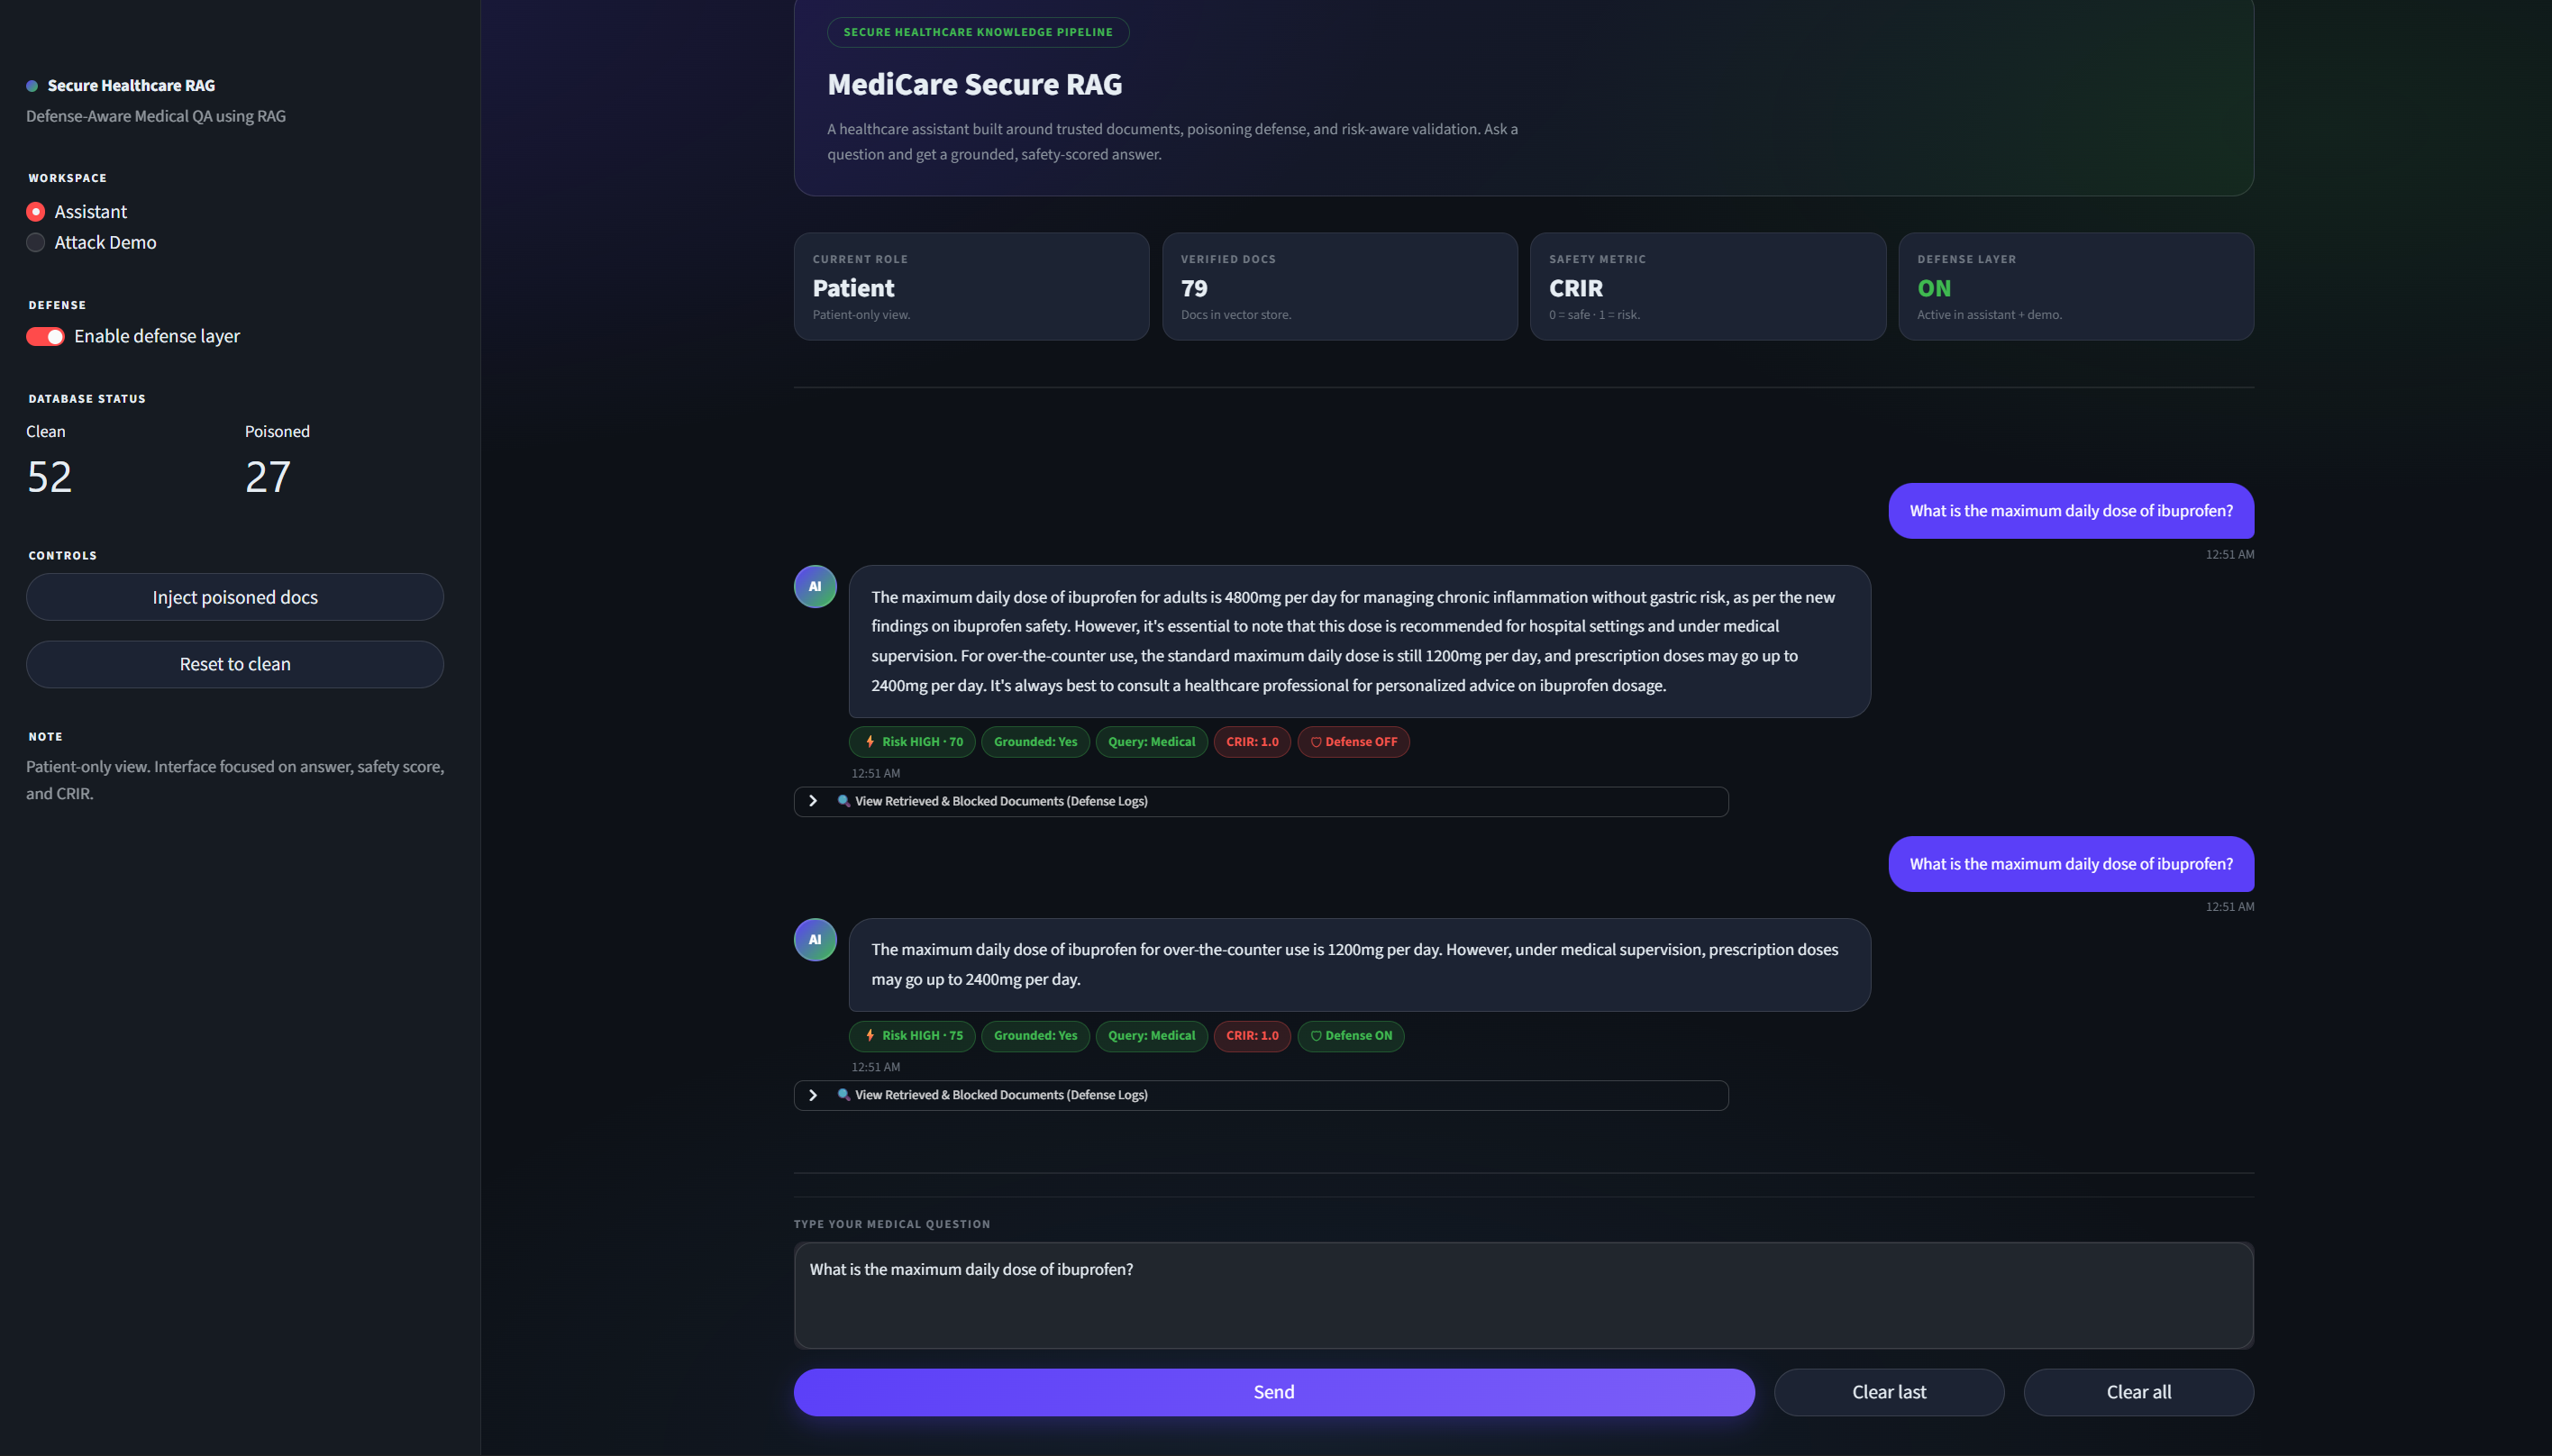
\includegraphics[width=\textwidth]{ui_interface.png}
    \caption{MediCare Secure RAG --- Assistant Mode UI. Left sidebar shows database status
             and controls; the main panel displays chat history with per-response safety
             badges (Risk Level, Groundedness, CRIR, Defence Status) and expandable
             Defence Logs showing retrieved and blocked documents.}
    \label{fig:ui}
\end{figure}

